\documentclass{article} % Tipo de documento
\usepackage[utf8]{inputenc} % Permite el uso de caracteres del Español
\usepackage[T1]{fontenc}
\usepackage{graphicx}
\usepackage{amsmath}
\usepackage{wrapfig}
\usepackage[top=1in, bottom=1.25in, left=1.1in, right=1.1in]{geometry}

% used in maketitle
\title{Reporte - Actividad 1}
\author{García Monge Itzel Alexia}
\date{30 de Enero, 2018}


%Vamos a iniciar el documento, empezando con los títulos
\begin{document}
\maketitle

\section{Introducción}
    El siguiente artículo ofrece una breve explicación sobre la atmosfera Terrestre, informando sobre la composición de sus gases, capas que la conforman, propiedades físicas como su masa y espesor, efectos ópticos, y la circulación que tiene el aire alrededor de esta.

\section{Composición}
	Los tres contituyentes más grandes del aire, y consecuentemente de la atmósfera Terrestre, son el Nitrogeno(78.084\%), Oxigeno(20.946) y Argón(0.9340). El resto de los gases, donde se encuentran los gases invernadero, son el Dioxido de Carbono(0.04\%), Neon(0.001818\%), Helio(0.000524\%) y Metano(0.000179\%). El aire filtrado contiene cantidades de otros componentes químicos como sustancias de origen natural o contaminantes industriales presentes localmente y por temporada en pequeñas cantidades.
    
    Además de tener gases en la atmósfera, también se cuenta con vapor de agua. La concentración de vapor de agua varía significativamente.Su porcentaje va de 1\% en la superficie terrestre y disminuye conforme aumenta la altitud hacia diferentes capas atmosféricas. La masa del vapor de agua se compone, cuando la temperatura es fría del 10\%, y cuando la temperatura es alta, del 5\% de la masa atmosférica total.

% para insertar una imágen solamente:
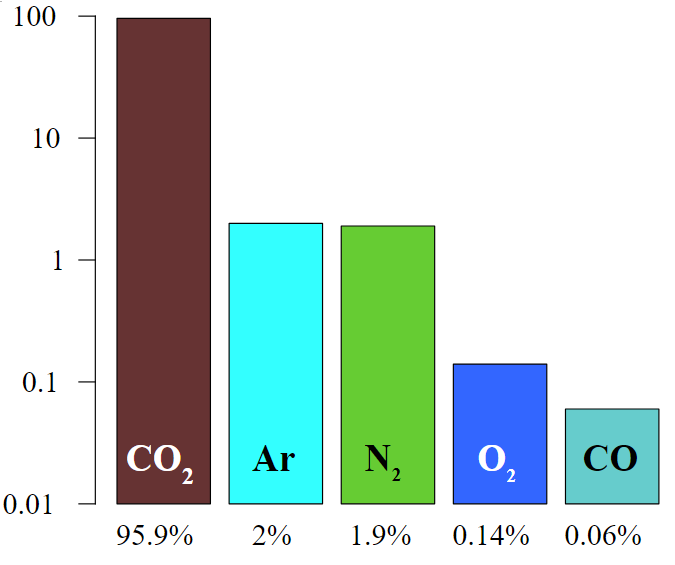
\includegraphics[height=8cm]{barra.png}{Porcentaje de Gases Atmosféricos}

\section{Estructuras de la Atmósfera}
	\subsection{Capas Principales}

% para insertar una imágen solamente:
%\includegraphics[height=10cm]{atmosfera.jpg}

%Para crear una imágen que pueda tener texto a los lados:
%\begin{wrapfigure}{c}{0.25\textwidth}
%	\centering
%    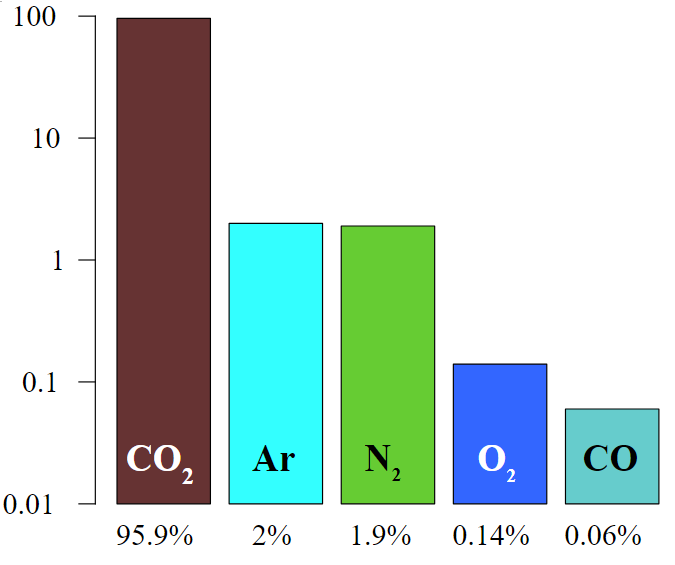
\includegraphics{barra.png}
%\end{wrapfigure}

El patrón general al medir la temperatura y altitud es constante y es medible por medio de instrumentos como los globos meteorológicos. El comportamiento de la temperatura provee una métrica útil para distinguir las capas atmosféricas, de esta manera, la atmósfera Terrestre puede dividirse en cinco principales capas.

    \subsubsection{Exosfera}
    La exosfera es la capa más exterior de la atmósfera Terrestre, extendiéndose desde una altitud de 700 hasta los 10,000 $km$ por arriba del nivel del mar. En esta capa orbitan la mayoría de los satélites de la Tierra.
    
    Esta compuesta principalmente por extremadamente bajas densidades de hidrógeno, helio y algunas otras moléculas más pesadas. Los átomos y moléculas están tan apartados entre si que pueden moverse por varios cientos de kilometros sin colisionar con otro. Por esto mismo, la exosfera no se comporta como un gas, y las partículas constantemente escapan al espacio exterior.
    
    \subsubsection{Termosfera}
    La Termosfera es la segunda capa más alta, se extiende a una altitud alrededor de 80 $km$ hasta un rango de altitud entre los 500 y 1,000 $km$.
    
    Su temperatura incrementa gradualmente con la altura, pues la inversión en la termosfera ocurre debido a la densidad extremadamente baja de sus moléculas. La temperatura puede subir tan alto como 1,500$\circ$C, pero las moléculas de gas están tan separadas que no se lograría sentir. EL aire está tan enrarecido que una molécula individual viaja 1 kilometro en promedio antes de colisionar con otra. 
    
	Está capa se encuentra completamente despejada y libre de vapor de agua. Sin embargo, fenómenos no hidrometeorológicos como las auroras borealis y australis pueden ser observados ocasionalmente. La Estación Espacial Internacional orbita en esta capa.
	
    \subsubsection{Mesosfera}
    La mesosfera es la tercera capa más alta de la atmosfera Terrestre, extendiéndose desde una altitud de 50 hasta los 80-85 $km$ por arriba del nivel del mar. Las temperaturas bajan entre más se incrementa la altitud hacia la mesopausa. Es el lugar más frío de la Tierra con una temperatura promedio de -85$\circ$C.
    
    Justo abajo de la mesopausa el aire es tan helado que el muy escaso vapor de agua puede ser sublimado en nubes noctilucentes polar-mesosféricas, estas son las nubes más altas de la atmósfera. La mesosfera también es la capa donde la mayoría de los meteorítos se queman al entrar a la atmósfera. 
    
    Está demasiado alto en la Tierra como para ser accesible para aeronaves y globos propulsados comúnmente, y demasiado bajo para permitir que orbiten naves espaciales. Esta capa es principalmente entrada por cohetes de sonido y aeronaves propulsadas por cohetes.
     
     \subsubsection{Estratosfera}
     La Estratosfera es la segunda capa más baja de la atmósfera Terrestre, se extiende aproximadamente a unos 12 $km$ por arriba de la superficie terrestre a una altitud alrededor de 50 a 55 $km$.
     
     La presión atmosférica ubicada arriba de la estratosfera es de aproximadamente 1/1,000 a la presión del nivel del mar. Contiene a la capa de ozono y define una capa en la cual las temperaturas se elevan entre más se suba de altitud, lo cual restrige la turbulencia. Consequentemente, la estratosfera esta casi completamente libre de nubes y otros tipos de clima.
     
     Es la capa más alta en la cual se puede acceder con una nave de propulsión a chorro.
     
     \subsubsection{Troposfera}
     La capa más baja de la Tierra, se extiende desde la supercifie Terrestre con una altura promedio de 12 $km$, aunque su altitud varíe desde los 9 $km$ en los polos, hasta 17 $km$ en el ecuador.
     
     Aunque variaciones por el clima pueden ocurrir, la temperatura usualmente baja entre más se incremente de altitud. Así, la parte más baja es típicamente la sección más cálida. La troposfera contiene aproximadamente 80\% de la masa de la atmósfera Terrestre, siendo también la más densa al tener un mayor peso atmoséfrico arriba de este. Cincuenta por ciento del total de la masa atmosférica se localiza abajo de los 5.6km.
     
     Casi todo el vapor de agua atmosférico o humedad se encuentra en la troposfera, así que es la capa donde casí todo el clima de la Tierra ocurre. Tiene todos los tipos de nubes asociados con el clima generadas por una circulación de viento activo. 
     
     La actividad de aviación más convencional tiene lugar en esta capa, y es la única que puede ingresarse por aviones propulsados por hélices.
     
     \subsubsection{Otras Capas}
     Dentro de las cinco capas principales que están determinadas en gran parte por temperatura, se encuentran capas que pueden ser separadas por otras propiedades:
     
\begin{itemize}
\item La capa de ozono está contenida en la estratosfera, alrededor del 90\% del ozono en la atmósfera Terrestre es contenida ahí. 
\item La ionosfera es una región de la atmósfera que está ionizada por radiación solar y es reponsable por las auroras.Además, forma el borde interior de la magnetósfera, la cual influye en la propagación de ondas de radio en la Tierra. 
\item El límite planetario es la parte de la troposfera que esta más cerca a la superficie Terrestre y es discretamente afectada por ella, principalmente por medio de difusión turbulenta. La profundidad del límite planetario va desde los 100 metros en noches tranquilas y despejadas, hasta los 3,000 metros o más durante las tardes en regiones secas.
\end{itemize}

%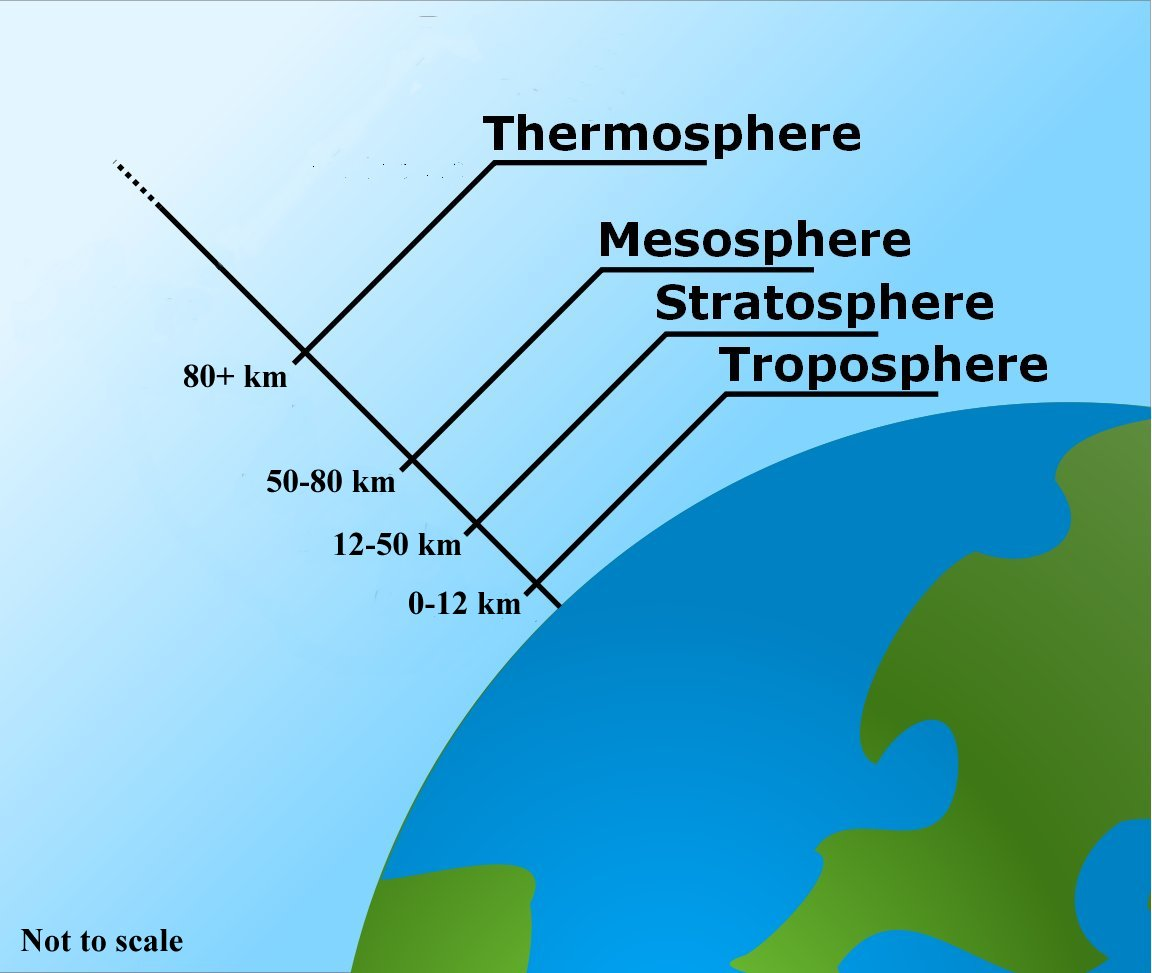
\includegraphics[height=8cm]{capas.jpg}{Capas de la Atmósfera}

\begin{figure}{Capas de la Atmósfera}
\centering
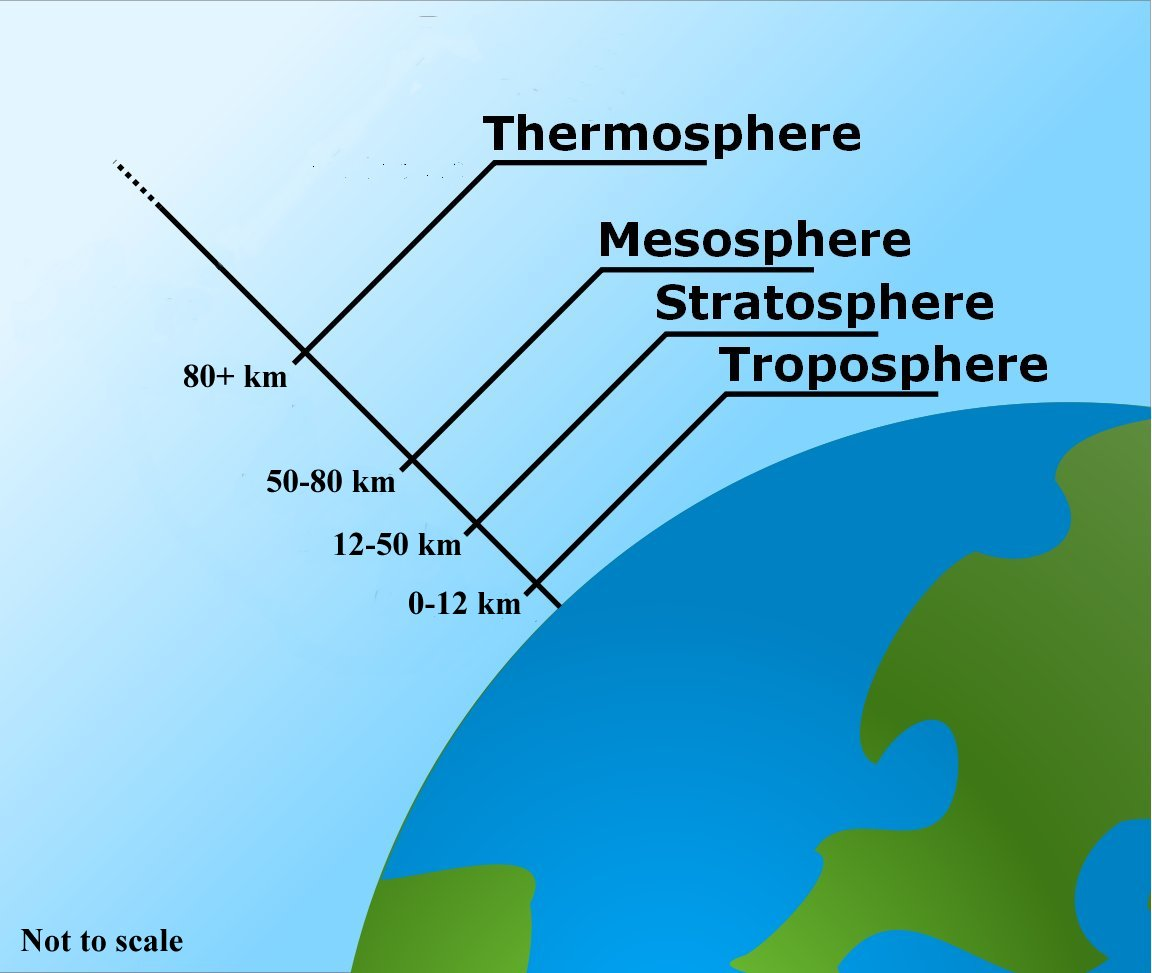
\includegraphics[height=8cm]{capas.jpg}
\end{figure}

\section{Propiedades Físicas}
	\subsection{Presión y Espesor}
   	La presión atmosférica es el peso total del aire arriba de una unidad de área en el punto donde la presión es medida y varía dependiendo de su locación y clima. La presión atmosférica promedio a nivel del mar es de 101,325 pascales, mientras que la masa atmosférica total es de 5.1480$\times10^{18} kg$.
    
    Si toda la masa de la atmósfera tuviera una densidad uniforme desde el nivel del mar, esta terminaría abruptamente en una altitud de 8.50 $km$. En realidad lo que ocurre es que va decresiendo exponencialmente con la altitud, bajando a la mitad cada 5.6 km o por un factor de 1/e cada 7.64 km. Sin embargo, la atmósfera es modelada de manera más precisa con una ecuación personalizada para cada capa, tomando en cuenta la temperatura, composición molecuclar y radiación solar.


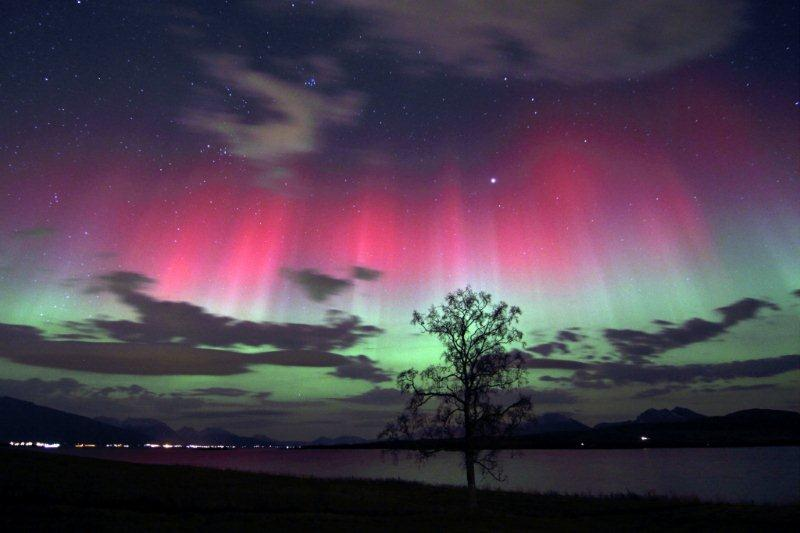
\includegraphics[height=10cm]{auroras.jpg}{Aurora Borealis}

	\subsection{Temperatura y Velocidad del Sonido}
     La temperatura disminuye entre más altitud se tome, empezando en el nivel del mar. Variaciones de esta moda empiezan arriba de los 11 $km$, donde la temperatura se estabiliza a través de una larga distancia vertical por el resto de la troposfera, para que nuevamente en la estratosfera la temperatura incremente con la altura.
     
	En un gas ideal de composición constante la velocidad del sonido depende solamente de la temperatura y no de la presión del gas o la densidad. La velocidad del sonido en la atmósfera con altitud toma forma de un perfil de temperatura complicado y no refleja cambios altitudinales en densidad ni presión.
	
    \subsection{Densidad y Masa}
    La densidad del aire no se mide directamente, sino que es calculada por mediciones a la temperatura, presión y humedad usando ecuaciones del estado del aire, obteniendo una densidad promedio a nivel del mar de 1.2 $\frac{kg}{m^3}$. La denisdad atmosférica disminuye conforme se incrememnta la altitud, esta variación puede ser modelada aproximadamente usando la fórmula barométrica, mientras que algunos modelos más sofisticados son usados para predecir el deterioro orbital de satélites. 
    
    La masa promedio de la atmósfera es cerca de 5 cuatrillón de toneladas la masa de la Tierra. Para poner una perspectiva: la Tierra es el planeta más denso del Sistema Solar, con una densidad de 5.513 $\frac{g}{cm^3}$, si se toma en cuenta la compresión gravitacional, el valor se calcula dividiendo la masa del planeta por su volumen..
     
\section{Propiedades Ópticas}
    La radiación solar es la energía que la Tierra recibe del Sol. La Tierra también emite radiación de vuelta al espacio, pero en longitudes de onda más largas que no podemos percibir. Ya sea radiación emitida o entrante, parte de ella es absorbida por la atmósfera. 
    
    \subsection{Dispersión}
    Cuando la luz pasa por la atmósfera Terrestre, fotones interactuan con ella por medio de la dispersión. Si la luz no interactuara con la atmósfera sería radiación directa, y es lo que vez si fueses a mirar directamente al Sol. La radiación indirecta es luz que ha sido dispersada en la atmósfera.
    
    Debido a un fenómeno llamadado Dispersión de Rayleigh, las longitudes de onda cortas se dispersan con mayor facilidad que longitudes de onda largas.
    
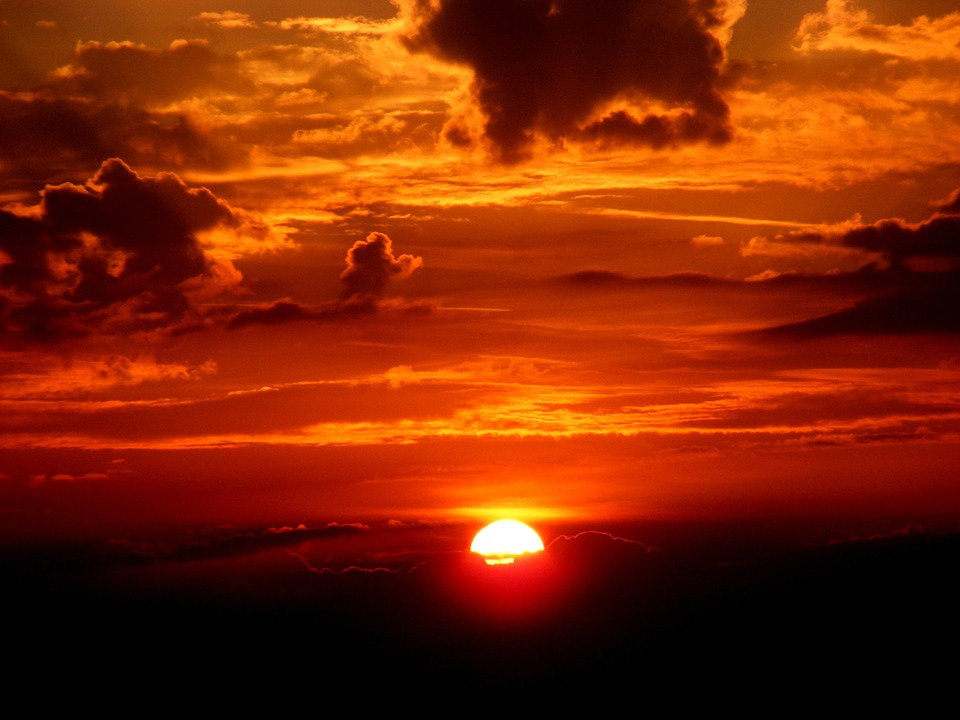
\includegraphics[height=8cm]{sunset.jpg}{Ejemplo de Dispersión}

    \subsection{Absorción}
    Diferentes moléculas absorben diferentes longitudes de radiación. Cuando una molécula abosrbe un fotón, esta incrementa la energía de la molécula, lo cual calienta la atmósfera. Esto se logra contrarrestar con el enfriamiento causado por la Tierra al emitir radiación.
    
    La absorción combinada de los gases en la atmósfera deja "ventanas" de opacidad baja permitiendo la transmisión de ciertas bandas de luz. La ventana óptica corre desde alrededor de 300 $nm$ hasta el espectro visible, comúnmente llamado luz, en aproximadamente 400-700 $nm$ y continua en el infrarrojo alrededor de los 1,100 $nm$.
    
    \subsection{Emisión}
    Emisión es cuando un objeto emite radiación; objetos tienden a emitir ciertas cantidades y radiación de longitudes de onda dependiendo de las curvas de emisión de su "cuerpo negro", por lo tanto, objetos más calientes tienden a emitir más radiación con longitudes de onda más cortas y vice versa.
    
    Por su temperatura, la atmósfera emite radiación infrarroja. El efecto invernadero está directamente relacionado con el efecto de absorción y emisión. Algunos gases en la atmósfera absorben y emiten radiación infrarroja, pero no interactuan con la luz solar en el espectro visible.

	\subsection{Índice de Refracción}
   	El índice de refracción del aire depende de la temperatura, dando lugar a los efectos de refracción cuando el gradiente de temperatura es largo. Variaciones sistemáticas en los índices de refracción pueden dirigir hacia la refracción de los rayos de luz sobre caminos ópticos largos.

\section{Circulación}
    La circulación atmosférica es el movimiento a gran escala de aire por la troposfera, y el medio por el cual el calor es distribuido alrededor de la Tierra. Esta estructura a gran escala de la circulación atmosférica varía año con año, pero la estructura básica se mantiene bastante constante ya que es determinado por el ritmo de rotación de la Tierra y la diferencia en radiación solar entre el ecuador y los polos.

\section{Ápendice}
\begin{enumerate}
\item ¿Qué fue lo que más te llamó la atención de esta actividad?
La forma en que podemos escribir las ecuaciones y dar formato al texto e imágenes de manera menos tediosa comparada con los procesadores de textos como Word y Google Docs.

\item ¿Qué fue lo que se te hizo menos interesante?
Buscar los paquetes para las imágenes, ya que hay varias de ellas y cada una logra hacer algo en especial con la imágen, entonces debía buscar un nuevo paquete si quería centrar la imágen o ponerla alrededor del texto, en lugar de usar el mismo paquete de manera más sencilla.

\item ¿Qué cambios harías para mejorar esta actividad? Dar una clase introductoría sobres los comandos de LaTeX, para qué sirven y un poco de ejemplos de cómo usarlos en actividades más cortas y en clase antes de dejar un trabajo de tal extensión sin saber nada sobre el programa y sus funciones.

\item ¿Cuál es tu primera impresión de uso de LATEX? Siento que es un procesador de textos orientado a los escritos científicos, ya que tiene muchos comandos que permiten un manejo relativamente sencillo de los símbolos usandos comúnmente en ellos. Aunque es desesperante lo lento que los procesadores de LaTeX tardan en mostrar los errores y lo que se ha escrito en su "preview".

\item ¿El tiempo sugerido para esta actividad fue suficiente? Lo fue para completar la actividad, pero siento que se necesitó más tiempo para comprender de manera conscisa el funcionamiento de los comandos y paquetes de LaTeX.

\item ¿Encontraste algún documento o recurso en línea útil que quisieras compartir con los demás?  La página Share LaTeX me ayudó en el formato del texto, así como el documento "A Quick Guide to LaTex". Sus links son:

$https://www.sharelatex.com/learn/List \# Ordered_lists$

$https://www.overleaf.com/latex/templates/a-quick-guide-to-latex/fghqpfgnxggz \# .WnAE_6jiZEY$
\end{enumerate} 

\section{Bibliografía}
\begin{itemize}
\item Atmosphere of Earth. (2018, January 28). Retrieved January 29, 2018, from

$https://en.wikipedia.org/wiki/Atmosphere_of_Earth $

\item Trace Gases. Retrieved January 29, 2018, from 

$https://web.archive.org/web/20101009044345/http://www.ace.mmu.ac.uk/eae/atmosphere/older/Trace_Gases.html$

\item Density of the Earth. (2015, December 24). Retrieved January 29, 2018, from 

$https://www.universetoday.com/26771/density-of-the-earth/$
\end{itemize}

\subsection{Imágenes}
\begin{itemize}
\item $https://upload.wikimedia.org/wikipedia/commons/2/27/PIA16460_Mars_Atmosphere_Gases_20121102.svg$
\item $https://upload.wikimedia.org/wikipedia/en/5/55/AtmosphericLayers.jpg$
\item $https://upload.wikimedia.org/wikipedia/commons/3/3f/Aurora_Borealis_I.jpg$
\item $https://pixabay.com/p-478396/?no_redirect$
\end{itemize}
\end{document}
